\documentclass{beamer}

%
% Common preamble for all three parts.
%


\usepackage{amsmath}
\usepackage{color}
\usepackage{minted}
\usepackage{hyperref}
\usepackage{multicol}
\usepackage{tabularx}
\usepackage{tikz}
\usepackage[utf8]{inputenc}
\usepackage[greek,english]{babel}

\newcommand{\en}{\selectlanguage{english}}
\newcommand{\gr}{\selectlanguage{greek}}

% only inline todonotes work
\usepackage{xkeyval}
\usepackage[textsize=small]{todonotes}
\presetkeys{todonotes}{inline}{}

\usetikzlibrary{shapes,arrows,positioning,shadows}

% no nav buttons
\usenavigationsymbolstemplate{}

\newcommand{\bftt}[1]{\textbf{\texttt{#1}}}
\newcommand{\comment}[1]{{\color[HTML]{008080}\textit{\textbf{\texttt{#1}}}}}
\newcommand{\cmd}[1]{{\color[HTML]{008000}\bftt{#1}}}
\newcommand{\bs}{\char`\\}
\newcommand{\cmdbs}[1]{\cmd{\bs#1}}
\newcommand{\lcb}{\char '173}
\newcommand{\rcb}{\char '175}
\newcommand{\cmdbegin}[1]{\cmdbs{begin\lcb}\bftt{#1}\cmd{\rcb}}
\newcommand{\cmdend}[1]{\cmdbs{end\lcb}\bftt{#1}\cmd{\rcb}}

\newcommand{\wllogo}{\textbf{Overleaf}}

% this is where the example source files are loaded from
% do not include a trailing slash
\newcommand{\fileuri}{https://raw.github.com/jdleesmiller/latex-course/master/en}

\newcommand{\wlserver}{https://www.overleaf.com}
\newcommand{\wlnewdoc}[1]{\wlserver/docs?snip\_uri=\fileuri/#1\&splash=none}

\def\tikzname{Ti\emph{k}Z}

% from http://tex.stackexchange.com/questions/5226/keyboard-font-for-latex
\newcommand*\keystroke[1]{%
  \tikz[baseline=(key.base)]
    \node[%
      draw,
      fill=white,
      drop shadow={shadow xshift=0.25ex,shadow yshift=-0.25ex,fill=black,opacity=0.75},
      rectangle,
      rounded corners=2pt,
      inner sep=1pt,
      line width=0.5pt,
      font=\scriptsize\sffamily
    ](key) {#1\strut}
  ;
}
\newcommand{\keystrokebftt}[1]{\keystroke{\bftt{#1}}}

% stolen from minted.dtx
\newenvironment{exampletwoup}
  {\VerbatimEnvironment
   \begin{VerbatimOut}{example.out}}
  {\end{VerbatimOut}
   \setlength{\parindent}{0pt}
   \fbox{\begin{tabular}{l|l}
   \begin{minipage}{0.55\linewidth}
     \inputminted[fontsize=\small,resetmargins]{latex}{example.out}
   \end{minipage} &
   \begin{minipage}{0.35\linewidth}
     \input{example.out}
   \end{minipage}
   \end{tabular}}}

\newenvironment{exampletwouptiny}
  {\VerbatimEnvironment
   \begin{VerbatimOut}{example.out}}
  {\end{VerbatimOut}
   \setlength{\parindent}{0pt}
   \fbox{\begin{tabular}{l|l}
   \begin{minipage}{0.55\linewidth}
     \inputminted[fontsize=\scriptsize,resetmargins]{latex}{example.out}
   \end{minipage} &
   \begin{minipage}{0.35\linewidth}
     \setlength{\parskip}{6pt plus 1pt minus 1pt}%
     \raggedright\scriptsize\input{example.out}
   \end{minipage}
   \end{tabular}}}

\newenvironment{exampletwouptinynoframe}
  {\VerbatimEnvironment
   \begin{VerbatimOut}{example.out}}
  {\end{VerbatimOut}
   \setlength{\parindent}{0pt}
   \begin{tabular}{l|l}
   \begin{minipage}{0.55\linewidth}
     \inputminted[fontsize=\scriptsize,resetmargins]{latex}{example.out}
   \end{minipage} &
   \begin{minipage}{0.35\linewidth}
     \setlength{\parskip}{6pt plus 1pt minus 1pt}%
     \raggedright\scriptsize\input{example.out}
   \end{minipage}
   \end{tabular}}

\title{ Μια διαδραστική εισαγωγή στο \LaTeX}

\author{\textlatin{Dr John D. Lees-Miller} \\ 
\small {Μετάφραση : Αθανάσιος Παρασκευόπουλος \\(μεταπτυχιακός φοιτητής του ΕΑΠ)}}

\titlegraphic{%

\includegraphics[height=36pt]{overleaf}\\[1em]

\includegraphics[height=24pt]{UoB-logo}
}

\gr
\subtitle{Part 3: Not Just Papers: Presentations \& More}

\newcommand{\alice}[1]{\todo[color=green!40]{#1}}
\newcommand{\bob}[1]{\todo[color=purple!40]{#1}}

\begin{document}
\gr
%%%%%%%%%%%%%%%%%%%%%%%%%%%%%%%%%%%%%%%%%%%%%%%%%%%%%%%%%%%%%%%%%%%%%%%%%%%%%%%
%%%%%%%%%%%%%%%%%%%%%%%%%%%%%%%%%%%%%%%%%%%%%%%%%%%%%%%%%%%%%%%%%%%%%%%%%%%%%%%
%%%%%%%%%%%%%%%%%%%%%%%%%%%%%%%%%%%%%%%%%%%%%%%%%%%%%%%%%%%%%%%%%%%%%%%%%%%%%%%
\begin{frame}
\titlepage
\end{frame}

%%%%%%%%%%%%%%%%%%%%%%%%%%%%%%%%%%%%%%%%%%%%%%%%%%%%%%%%%%%%%%%%%%%%%%%%%%%%%%%
%%%%%%%%%%%%%%%%%%%%%%%%%%%%%%%%%%%%%%%%%%%%%%%%%%%%%%%%%%%%%%%%%%%%%%%%%%%%%%%
%%%%%%%%%%%%%%%%%%%%%%%%%%%%%%%%%%%%%%%%%%%%%%%%%%%%%%%%%%%%%%%%%%%%%%%%%%%%%%%
%\begin{frame}{Setup}
%\begin{itemize}
%\item Go to this URL in Google Chrome (\emph{not} Internet Explorer) to open
%these slides on your computer:
%\vskip 2em
%\begin{center}
%\fbox{\url{http://bit.ly/12WWWqj}}
%\end{center}
%\vskip 2em
%\item Here are the slides from the previous tutorial, for reference:
%\begin{center}
%\vskip 1em
%\fbox{\href{https://dl.dropboxusercontent.com/u/31383671/site/latex_course_v2/part1.pdf}{Part 1: The Basics}}
%\vskip 1em
%\fbox{\href{https://dl.dropboxusercontent.com/u/31383671/site/latex_course_v2/part2.pdf}{Part 2: Structured Documents \& More}}
%\end{center}
%\end{itemize}
%\end{frame}

%%%%%%%%%%%%%%%%%%%%%%%%%%%%%%%%%%%%%%%%%%%%%%%%%%%%%%%%%%%%%%%%%%%%%%%%%%%%%%%
%%%%%%%%%%%%%%%%%%%%%%%%%%%%%%%%%%%%%%%%%%%%%%%%%%%%%%%%%%%%%%%%%%%%%%%%%%%%%%%
%%%%%%%%%%%%%%%%%%%%%%%%%%%%%%%%%%%%%%%%%%%%%%%%%%%%%%%%%%%%%%%%%%%%%%%%%%%%%%%
\section{Ανακεφαλαίωση \LaTeX{}}

%%%%%%%%%%%%%%%%%%%%%%%%%%%%%%%%%%%%%%%%%%%%%%%%%%%%%%%%%%%%%%%%%%%%%%%%%%%%%%%
%%%%%%%%%%%%%%%%%%%%%%%%%%%%%%%%%%%%%%%%%%%%%%%%%%%%%%%%%%%%%%%%%%%%%%%%%%%%%%%
%%%%%%%%%%%%%%%%%%%%%%%%%%%%%%%%%%%%%%%%%%%%%%%%%%%%%%%%%%%%%%%%%%%%%%%%%%%%%%%
\begin{frame}[fragile]{\insertsection}
\begin{itemize}
\item  Γράφετε το έγγραφό σας σε \texttt{απλό κείμενο} με \cmd{εντολές} που περιγράφουν τη δομή και το νόημά του.
\item Το πρόγραμμα \en \texttt{latex} \gr επεξεργάζεται το κείμενο και τις εντολές σας για να δημιουργήσει ένα
όμορφα διαμορφωμένο έγγραφο.
\end{itemize}
\vskip 2ex
\en
\begin{center}
\begin{minted}[frame=single]{latex}
The rain in Spain falls \emph{mainly} on the plain.
\end{minted}
\vskip 2ex
\tikz\node[single arrow,fill=gray,font=\ttfamily\bfseries,%
  rotate=270,xshift=-1em]{latex};
\vskip 2ex
\fbox{The rain in Spain falls \emph{mainly} on the plain.}
\end{center}
\end{frame}
\gr
%%%%%%%%%%%%%%%%%%%%%%%%%%%%%%%%%%%%%%%%%%%%%%%%%%%%%%%%%%%%%%%%%%%%%%%%%%%%%%%
%%%%%%%%%%%%%%%%%%%%%%%%%%%%%%%%%%%%%%%%%%%%%%%%%%%%%%%%%%%%%%%%%%%%%%%%%%%%%%%
%%%%%%%%%%%%%%%%%%%%%%%%%%%%%%%%%%%%%%%%%%%%%%%%%%%%%%%%%%%%%%%%%%%%%%%%%%%%%%%
\begin{frame}[fragile]{\insertsection: Εντολές και Ορίσματα}
\begin{itemize}
\item Μια εντολή ξεκινά με \en\emph{backslash} \keystrokebftt{\bs}\gr.
\item Ορισμένες εντολές λαμβάνουν ένα \emph{όρισμα} σε σγουρά άγκιστρα \en \keystrokebftt{\{}
\keystrokebftt{\}}\gr.
\item Ορισμένες εντολές λαμβάνουν επίσης \emph{προαιρετικά ορίσματα} σε αγκύλες \en\keystrokebftt{[} \keystrokebftt{]}\gr.
\end{itemize}
\vskip 2ex
\en
\begin{exampletwouptiny}

\includegraphics[
  width=0.5\textwidth]{gerbil}


\includegraphics[
  width=0.3\textwidth,
  angle=270]{gerbil}
\end{exampletwouptiny}

\tiny{Image license: \href{https://pixabay.com/en/animal-apple-attractive-beautiful-1239390/}{CC0}}

\end{frame}
\gr
%%%%%%%%%%%%%%%%%%%%%%%%%%%%%%%%%%%%%%%%%%%%%%%%%%%%%%%%%%%%%%%%%%%%%%%%%%%%%%%
%%%%%%%%%%%%%%%%%%%%%%%%%%%%%%%%%%%%%%%%%%%%%%%%%%%%%%%%%%%%%%%%%%%%%%%%%%%%%%%
%%%%%%%%%%%%%%%%%%%%%%%%%%%%%%%%%%%%%%%%%%%%%%%%%%%%%%%%%%%%%%%%%%%%%%%%%%%%%%%
\begin{frame}[fragile]{\insertsection: Περιβάλλοντα}
\begin{itemize}
\item Οι εντολές \en \cmdbs{begin}\gr \space και \en \cmdbs{end} \gr χρησιμοποιούνται για τη δημιουργία πολλών διαφορετικών περιβαλλόντων

\item Τα περιβάλλοντα \en \bftt{itemize}\gr \spaceκαι \en \bftt{enumerate} \gr δημιουργούν λίστες.
\vskip 2ex
\en
\begin{exampletwouptiny}
\begin{itemize} % for bullet points
\item Biscuits
\item Tea
\end{itemize}

\begin{enumerate} % for numbers
\item Biscuits
\item Tea
\end{enumerate}
\end{exampletwouptiny}

\end{itemize}
\end{frame}
\gr
%%%%%%%%%%%%%%%%%%%%%%%%%%%%%%%%%%%%%%%%%%%%%%%%%%%%%%%%%%%%%%%%%%%%%%%%%%%%%%%
%%%%%%%%%%%%%%%%%%%%%%%%%%%%%%%%%%%%%%%%%%%%%%%%%%%%%%%%%%%%%%%%%%%%%%%%%%%%%%%
%%%%%%%%%%%%%%%%%%%%%%%%%%%%%%%%%%%%%%%%%%%%%%%%%%%%%%%%%%%%%%%%%%%%%%%%%%%%%%%
\begin{frame}[fragile]{\insertsection: Μαθηματικά}
\begin{itemize}
\item Το περιβάλλον \en \bftt{equation} \gr δημιουργεί μια αριθμημένη εξίσωση.
\en
\begin{exampletwouptiny}
\begin{equation}
  \sum_{k=1}^{n} \frac{1}{2^k}
\end{equation}
\end{exampletwouptiny}
\vskip 2ex
\gr
\item Χρησιμοποιήστε τo δολάριο \en \keystrokebftt{\$} \gr για να εισάγετε μαθηματικά.\\[1ex]
\en
\begin{exampletwouptiny}
% not so good:
Let a and b be distinct positive
integers, and let c = a - b + 1.

% much better:
Let $a$ and $b$ be distinct positive
integers, and let $c = a - b + 1$.
\end{exampletwouptiny}
\gr
\vskip 2ex
\item Χρησιμοποιείτε πάντα σύμβολα του δολαρίου σε ζευγάρια --- ένα για να ξεκινήσετε τα μαθηματικά και ένα για να τα τελειώσετε.
\vskip 1em
{\scriptsize Στην πραγματικότητα, θα μπορούσαμε να έχουμε γράψει \en \bftt{\$...\$} \gr ως
\en \cmdbegin{math}\bftt{...}\cmdend{math}.} \gr
\end{itemize}
\end{frame}

%%%%%%%%%%%%%%%%%%%%%%%%%%%%%%%%%%%%%%%%%%%%%%%%%%%%%%%%%%%%%%%%%%%%%%%%%%%%%%%
%%%%%%%%%%%%%%%%%%%%%%%%%%%%%%%%%%%%%%%%%%%%%%%%%%%%%%%%%%%%%%%%%%%%%%%%%%%%%%%
%%%%%%%%%%%%%%%%%%%%%%%%%%%%%%%%%%%%%%%%%%%%%%%%%%%%%%%%%%%%%%%%%%%%%%%%%%%%%%%
\begin{frame}[fragile]{\insertsection: Δομή Εγγράφου}
\begin{itemize}{\small
\item Ξεκινά με το \en \cmdbs{documentclass} \gr --- τι τύπο εγγράφου.
\item Μεταδεδομένα \en (\cmdbs{title} \gr και \en \cmdbs{author})\gr και πακέτα στο
προοίμιο.
\item Περιεχόμενο μεταξύ \en \cmdbegin{document}\gr και \en \cmdend{document} \gr.
\item Η εντολή \en \cmdbs{maketitle}\gr δημιουργεί τον τίτλο. Οι εντολές \en \cmdbs{section} \gr δημιουργούν αριθμημένες ενότητες.
}\end{itemize}
\en
\begin{minipage}{0.55\linewidth}
\inputminted[fontsize=\scriptsize,frame=single,resetmargins]{latex}%
  {recap-structure.tex}
\end{minipage}
\begin{minipage}{0.35\linewidth}
% trim: l b r t

\includegraphics[width=\textwidth,clip,trim=1.5in 7in 3in 2in]{recap-structure.pdf}
\end{minipage}
\end{frame}
\gr
%%%%%%%%%%%%%%%%%%%%%%%%%%%%%%%%%%%%%%%%%%%%%%%%%%%%%%%%%%%%%%%%%%%%%%%%%%%%%%%
%%%%%%%%%%%%%%%%%%%%%%%%%%%%%%%%%%%%%%%%%%%%%%%%%%%%%%%%%%%%%%%%%%%%%%%%%%%%%%%
%%%%%%%%%%%%%%%%%%%%%%%%%%%%%%%%%%%%%%%%%%%%%%%%%%%%%%%%%%%%%%%%%%%%%%%%%%%%%%%
\begin{frame}[fragile]{\insertsection: Άσκηση}

\begin{enumerate}
\item Ακολουθεί το κείμενο για ένα σύντομο άρθρο:\footnote{Βασισμένο στο \en \url{http://www.cgd.ucar.edu/cms/agu/scientific_talk.html}}\gr
\begin{center}
\fbox{\href{\wlnewdoc{recap-exercise.tex}}{%
Κάντε κλικ για να ανοίξετε αυτήν την άσκηση \en \wllogo{}}}\gr
\end{center}
\vskip 2ex
\item Προσθέστε εντολές \LaTeX{} στο κείμενο για να μοιάζει με αυτό:
\begin{center}
\fbox{\href{\fileuri/recap-exercise-solution.pdf}\gr τοις εκατό, πληκτολογείστε \en (\cmdbs{\%})\gr.
\item Για να γράψετε την εξίσωση, χρησιμοποιήστε \en \cmdbs{frac} \gr για το κλάσμα και τις εντολές \en \cmdbs{left(} \gr και \en \cmdbs{right)}\gr για τις παρενθέσεις.
\end{itemize}
\end{block}
\end{frame}

%%%%%%%%%%%%%%%%%%%%%%%%%%%%%%%%%%%%%%%%%%%%%%%%%%%%%%%%%%%%%%%%%%%%%%%%%%%%%%%
%%%%%%%%%%%%%%%%%%%%%%%%%%%%%%%%%%%%%%%%%%%%%%%%%%%%%%%%%%%%%%%%%%%%%%%%%%%%%%%
%%%%%%%%%%%%%%%%%%%%%%%%%%%%%%%%%%%%%%%%%%%%%%%%%%%%%%%%%%%%%%%%%%%%%%%%%%%%%%%
\section{Παρουσιάσεις με \en\protect\bftt{beamer}\gr}

%%%%%%%%%%%%%%%%%%%%%%%%%%%%%%%%%%%%%%%%%%%%%%%%%%%%%%%%%%%%%%%%%%%%%%%%%%%%%%%
%%%%%%%%%%%%%%%%%%%%%%%%%%%%%%%%%%%%%%%%%%%%%%%%%%%%%%%%%%%%%%%%%%%%%%%%%%%%%%%
%%%%%%%%%%%%%%%%%%%%%%%%%%%%%%%%%%%%%%%%%%%%%%%%%%%%%%%%%%%%%%%%%%%%%%%%%%%%%%%
\begin{frame}[fragile]{\insertsection}
\begin{itemize}
\item Το \en Beamer \gr \spaceείναι ένα πακέτο για τη δημιουργία παρουσιάσεων (όπως αυτή!) στο \LaTeX{}.
\item Παρέχει την κλάση εγγράφων \en \bftt{beamer} \gr.
\item Χρησιμοποιήστε το περιβάλλον \en \bftt{frame} \gr για να δημιουργήσετε διαφάνειες.
\end{itemize}
\en
\begin{minipage}{0.55\linewidth}
\inputminted[fontsize=\scriptsize,frame=single,resetmargins]{latex}%
  {beamer-minimal.tex}
\end{minipage}
\begin{minipage}{0.35\linewidth}
% trim: l b r t

\includegraphics[width=\textwidth,clip,trim=1in 1in 1in 1in]{beamer-minimal.pdf}
\end{minipage}
\end{frame}
\gr
%%%%%%%%%%%%%%%%%%%%%%%%%%%%%%%%%%%%%%%%%%%%%%%%%%%%%%%%%%%%%%%%%%%%%%%%%%%%%%%
%%%%%%%%%%%%%%%%%%%%%%%%%%%%%%%%%%%%%%%%%%%%%%%%%%%%%%%%%%%%%%%%%%%%%%%%%%%%%%%
%%%%%%%%%%%%%%%%%%%%%%%%%%%%%%%%%%%%%%%%%%%%%%%%%%%%%%%%%%%%%%%%%%%%%%%%%%%%%%%
\begin{frame}[fragile]{\insertsection: Προχωρώντας}

\begin{itemize}
\item Καθώς προχωράμε στις ακόλουθες διαφάνειες, δοκιμάστε τα παραδείγματα πληκτρολογώντας τα στο παραδειγματικό έγγραφο στο \en \wllogo.\gr
\end{itemize}
\vskip 2ex
\begin{center}
\fbox{\href{\wlnewdoc{beamer-minimal.tex}}{%
Κάντε κλικ για να ανοίξετε το παράδειγμα  στο \en \wllogo{}}}\gr
\end{center}
\end{frame}

%%%%%%%%%%%%%%%%%%%%%%%%%%%%%%%%%%%%%%%%%%%%%%%%%%%%%%%%%%%%%%%%%%%%%%%%%%%%%%%
%%%%%%%%%%%%%%%%%%%%%%%%%%%%%%%%%%%%%%%%%%%%%%%%%%%%%%%%%%%%%%%%%%%%%%%%%%%%%%%
%%%%%%%%%%%%%%%%%%%%%%%%%%%%%%%%%%%%%%%%%%%%%%%%%%%%%%%%%%%%%%%%%%%%%%%%%%%%%%%
\begin{frame}[fragile]
\frametitle{\insertsection: \en Frames \gr}
\begin{itemize}
\item Χρησιμοποιήστε το \en \cmdbs{frametitle} \gr για να δώσετε στη διαφάνεια έναν τίτλο.
\item Στη συνέχεια, προσθέστε περιεχόμενο στη διαφάνεια.
\item Ο κώδικας για αυτή την διαφάνεια μοιάζει με αυτό:
\vskip 2ex
\en
\inputminted[fontsize=\scriptsize,frame=single,resetmargins]{latex}%
  {beamer-frame.tex}
\end{itemize}
\end{frame}
\gr
%%%%%%%%%%%%%%%%%%%%%%%%%%%%%%%%%%%%%%%%%%%%%%%%%%%%%%%%%%%%%%%%%%%%%%%%%%%%%%%
%%%%%%%%%%%%%%%%%%%%%%%%%%%%%%%%%%%%%%%%%%%%%%%%%%%%%%%%%%%%%%%%%%%%%%%%%%%%%%%
%%%%%%%%%%%%%%%%%%%%%%%%%%%%%%%%%%%%%%%%%%%%%%%%%%%%%%%%%%%%%%%%%%%%%%%%%%%%%%%
\begin{frame}[fragile]{\insertsection: Ενότητες}
\begin{itemize}
\item Μπορείτε να χρησιμοποιήσετε το \en \cmdbs{section}s\gr για να ομαδοποιήσετε τις \bftt{διαφάνειες} σας και το \en \bftt{beamer} \gr θα το χρησιμοποιήσει για να δημιουργήσει αυτόματα μια περίληψη.
\item Για να δημιουργήσετε ένα περίγραμμα, χρησιμοποιήστε την εντολή \en \cmdbs{tableofcontents}\gr. Εδώ για αυτήν την παρουσίαση η επιλογή \en \bftt{currentsection}\gr επισημαίνει την τρέχουσα ενότητα.
\vskip 2ex
\en
\begin{exampletwouptiny}
\tableofcontents[currentsection]
\end{exampletwouptiny}
\end{itemize}
\end{frame}
\gr
%%%%%%%%%%%%%%%%%%%%%%%%%%%%%%%%%%%%%%%%%%%%%%%%%%%%%%%%%%%%%%%%%%%%%%%%%%%%%%%
%%%%%%%%%%%%%%%%%%%%%%%%%%%%%%%%%%%%%%%%%%%%%%%%%%%%%%%%%%%%%%%%%%%%%%%%%%%%%%%
%%%%%%%%%%%%%%%%%%%%%%%%%%%%%%%%%%%%%%%%%%%%%%%%%%%%%%%%%%%%%%%%%%%%%%%%%%%%%%%
\begin{frame}[fragile]{\insertsection: Πολλαπλές στήλες}
\begin{columns}
\begin{column}{0.4\textwidth}
\begin{itemize}
\item Χρησιμοποιήστε τα περιβάλλοντα \en \bftt{columns}\gr και \en \bftt{column}\gr για να σπάσετε τη διαφάνεια
σε στήλες.
\item Το όρισμα για κάθε \bftt{στήλη} καθορίζει το πλάτος της.
\item Δείτε επίσης το πακέτο \en \bftt{multicol}\gr, το οποίο σας σπάει αυτόματα
περιεχόμενο σε στήλες.
\end{itemize}
\end{column}
\en
\begin{column}{0.6\textwidth}
\begin{minted}[fontsize=\scriptsize,frame=single]{latex}
\begin{columns}
  \begin{column}{0.4\textwidth}
    \begin{itemize}
    \item Use the columns ...
    \item The argument ...
    \item See also the ...
    \end{itemize}
  \end{column}
  \begin{column}{0.6\textwidth}
    % second column
  \end{column}
\end{columns}
\end{minted}
\end{column}
\end{columns}
\end{frame}

%%%%%%%%%%%%%%%%%%%%%%%%%%%%%%%%%%%%%%%%%%%%%%%%%%%%%%%%%%%%%%%%%%%%%%%%%%%%%%%
%%%%%%%%%%%%%%%%%%%%%%%%%%%%%%%%%%%%%%%%%%%%%%%%%%%%%%%%%%%%%%%%%%%%%%%%%%%%%%%
%%%%%%%%%%%%%%%%%%%%%%%%%%%%%%%%%%%%%%%%%%%%%%%%%%%%%%%%%%%%%%%%%%%%%%%%%%%%%%%
\begin{frame}[fragile]{\insertsection: \en Highlights\gr}
\begin{itemize}

\item Χρησιμοποιήστε το \en \cmdbs{emph} \gr ή το \en \cmdbs{alert} \gr για να επισημάνετε:
\vskip 1ex \en
\begin{exampletwouptiny}
I should \emph{emphasise} that
this is an \alert{important} point.
\end{exampletwouptiny}
\vskip 1ex\gr

\item Ή καθορίστε έντονους χαρακτήρες ή πλάγιους χαρακτήρες:\en
\vskip 1ex
\begin{exampletwouptiny}
Text in \textbf{bold face}.
Text in \textit{italics}.
\end{exampletwouptiny}
\gr
\vskip 1ex

\item Ή καθορίστε ένα \en color \gr (αμερικανική ορθογραφία):
\vskip 1ex \en
\begin{exampletwouptiny}
It \textcolor{red}{stops}
and \textcolor{green}{starts}.
\end{exampletwouptiny}
\vskip 1ex\gr
\item Δείτε επίσης στο \en \url{http://www.math.umbc.edu/~rouben/beamer/quickstart-Z-H-25.html}\gr
για περισσότερα χρώματα \& προσαρμοσμένα χρώματα.
\end{itemize}
\end{frame}

%%%%%%%%%%%%%%%%%%%%%%%%%%%%%%%%%%%%%%%%%%%%%%%%%%%%%%%%%%%%%%%%%%%%%%%%%%%%%%%
%%%%%%%%%%%%%%%%%%%%%%%%%%%%%%%%%%%%%%%%%%%%%%%%%%%%%%%%%%%%%%%%%%%%%%%%%%%%%%%
%%%%%%%%%%%%%%%%%%%%%%%%%%%%%%%%%%%%%%%%%%%%%%%%%%%%%%%%%%%%%%%%%%%%%%%%%%%%%%%
\begin{frame}[fragile]{\insertsection: Σχήματα}
\begin{itemize}
\item Χρησιμοποιήστε το \en \cmdbs{includegraphics}\gr \space από το πακέτο \en \bftt{graphicx}\gr.
\item Το περιβάλλον \en\bftt{figure}\gr \space κεντράρεται από προεπιλογή, στο \en \bftt{beamer}\gr.
\vskip 2ex\en
\begin{exampletwouptiny}
\begin{figure}

\includegraphics[
  width=0.5\textwidth]{gerbil}
\end{figure}
\end{exampletwouptiny}
\end{itemize}
\en
\tiny{Image license: \href{https://pixabay.com/en/animal-apple-attractive-beautiful-1239390/}{CC0}}
\end{frame}
\gr
%%%%%%%%%%%%%%%%%%%%%%%%%%%%%%%%%%%%%%%%%%%%%%%%%%%%%%%%%%%%%%%%%%%%%%%%%%%%%%%
%%%%%%%%%%%%%%%%%%%%%%%%%%%%%%%%%%%%%%%%%%%%%%%%%%%%%%%%%%%%%%%%%%%%%%%%%%%%%%%
%%%%%%%%%%%%%%%%%%%%%%%%%%%%%%%%%%%%%%%%%%%%%%%%%%%%%%%%%%%%%%%%%%%%%%%%%%%%%%%
\begin{frame}[fragile]{\insertsection: Πίνακες}
\begin{itemize}
\item Οι πίνακες στο \LaTeX{} χρειάζονται λίγη εξοικείωση.
\item Χρησιμοποιήστε το περιβάλλον \en \bftt{tabular}\gr \space από το πακέτο \en\bftt{tabularx}\gr.
\item Το όρισμα καθορίζει τη στοίχιση στηλών ---\en \textbf{l}eft, \textbf{r}right, \textbf{r}right.\gr
\en
\begin{exampletwouptiny}
\begin{tabular}{lrr}
Item   & Qty & Unit \$ \\
Widget & 1   & 199.99  \\
Gadget & 2   & 399.99  \\
Cable  & 3   & 19.99   \\
\end{tabular}
\end{exampletwouptiny}
\gr
\item Χρησιμοποιήστε το \en\cmdbs{hline}\gr \space για οριζόντιες γραμμές.
\en
\begin{exampletwouptiny}
\begin{tabular}{|l|r|r|} \hline
Item   & Qty & Unit \$ \\\hline
Widget & 1   & 199.99  \\
Gadget & 2   & 399.99  \\
Cable  & 3   & 19.99   \\\hline
\end{tabular}
\end{exampletwouptiny}
\gr
\item Χρησιμοποιήστε ένα σύμφωνο \en \keystrokebftt{\&}\gr για να διαχωρίσετε στήλες και μια διπλή κάθετο \en \keystrokebftt{\bs}\keystrokebftt{\bs}\gr για να ξεκινήσετε μια νέα σειρά.
\end{itemize}
\end{frame}

%%%%%%%%%%%%%%%%%%%%%%%%%%%%%%%%%%%%%%%%%%%%%%%%%%%%%%%%%%%%%%%%%%%%%%%%%%%%%%%
%%%%%%%%%%%%%%%%%%%%%%%%%%%%%%%%%%%%%%%%%%%%%%%%%%%%%%%%%%%%%%%%%%%%%%%%%%%%%%%
%%%%%%%%%%%%%%%%%%%%%%%%%%%%%%%%%%%%%%%%%%%%%%%%%%%%%%%%%%%%%%%%%%%%%%%%%%%%%%%
\begin{frame}[fragile]{\insertsection: \en Blocks \gr}
\begin{itemize}
\item Ένα περιβάλλον \en \bftt{block}\gr δημιουργεί μια διαφάνεια με τίτλο.
\en
\begin{exampletwouptiny}
\begin{block}{Interesting Fact}
This is important.
\end{block}

\begin{alertblock}{Cautionary Tale}
This is really important!
\end{alertblock}
\end{exampletwouptiny}
\gr
\item Το πώς ακριβώς φαίνονται εξαρτάται από το θέμα\ldots
\end{itemize}
\end{frame}

%%%%%%%%%%%%%%%%%%%%%%%%%%%%%%%%%%%%%%%%%%%%%%%%%%%%%%%%%%%%%%%%%%%%%%%%%%%%%%%
%%%%%%%%%%%%%%%%%%%%%%%%%%%%%%%%%%%%%%%%%%%%%%%%%%%%%%%%%%%%%%%%%%%%%%%%%%%%%%%
%%%%%%%%%%%%%%%%%%%%%%%%%%%%%%%%%%%%%%%%%%%%%%%%%%%%%%%%%%%%%%%%%%%%%%%%%%%%%%%
\begin{frame}[fragile]
\frametitle{\insertsection: Θέματα}
\begin{itemize}
\item Προσαρμόστε την εμφάνιση της παρουσίασής σας χρησιμοποιώντας θέματα.
\item Δείτε εδώ \en \url{http://deic.uab.es/~iblanes/beamer_gallery/index_by_theme.html}\gr \space
για μια μεγάλη συλλογή θεμάτω
\end{itemize}
\en
\begin{minipage}{0.55\linewidth}
\inputminted[fontsize=\scriptsize,frame=single,resetmargins]{latex}%
  {beamer-theme.tex}
\end{minipage}
\begin{minipage}{0.35\linewidth}
% trim: l b r t
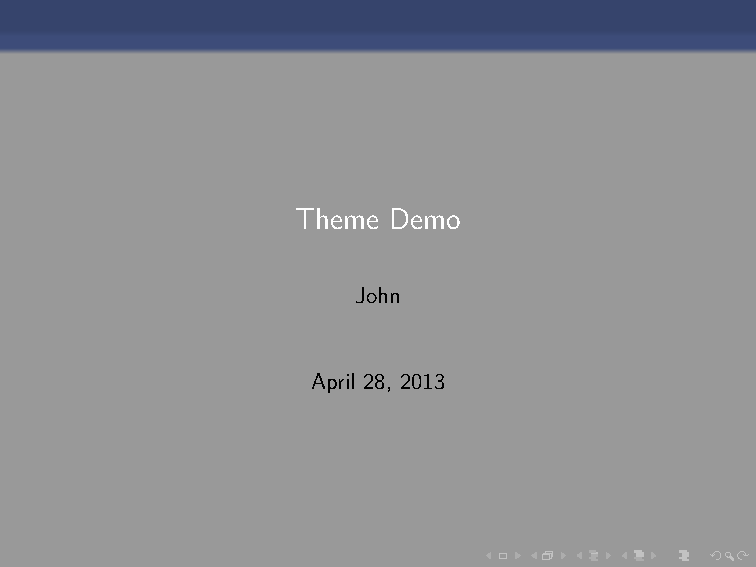
\includegraphics[width=\textwidth]{beamer-theme.pdf}
\end{minipage}
\end{frame}
\gr
%%%%%%%%%%%%%%%%%%%%%%%%%%%%%%%%%%%%%%%%%%%%%%%%%%%%%%%%%%%%%%%%%%%%%%%%%%%%%%%
%%%%%%%%%%%%%%%%%%%%%%%%%%%%%%%%%%%%%%%%%%%%%%%%%%%%%%%%%%%%%%%%%%%%%%%%%%%%%%%
%%%%%%%%%%%%%%%%%%%%%%%%%%%%%%%%%%%%%%%%%%%%%%%%%%%%%%%%%%%%%%%%%%%%%%%%%%%%%%%
\begin{frame}[fragile]{\insertsection: Κινουμένα γραφικά}
\begin{itemize}
\item Ένα \en frame\gr \space μπορεί να δημιουργήσει πολλές διαφάνειες.
\item Χρησιμοποιήστε την εντολή \en \cmdbs{pause}\gr \space για να εμφανίσετε μόνο μέρος μιας διαφάνειας.
\vskip 2ex
\en
\begin{exampletwouptinynoframe}
\begin{itemize}
\item Can you feel the 
\pause \item anticipation?
\end{itemize}
\end{exampletwouptinynoframe}
\vskip 2ex
\item There many more clever ways of making animations in \bftt{beamer}; see
also the \cmdbs{only}, \cmdbs{alt}, and \cmdbs{uncover} commands.
\end{itemize}
\end{frame}
\gr

%%%%%%%%%%%%%%%%%%%%%%%%%%%%%%%%%%%%%%%%%%%%%%%%%%%%%%%%%%%%%%%%%%%%%%%%%%%%%%%
%%%%%%%%%%%%%%%%%%%%%%%%%%%%%%%%%%%%%%%%%%%%%%%%%%%%%%%%%%%%%%%%%%%%%%%%%%%%%%%
%%%%%%%%%%%%%%%%%%%%%%%%%%%%%%%%%%%%%%%%%%%%%%%%%%%%%%%%%%%%%%%%%%%%%%%%%%%%%%%
\begin{frame}[fragile]{\insertsection: Άσκηση}

Δημιουργήστε ξανά την εξαιρετική «παρουσίαση \en Powerpoint Gettysburg\gr» του \en Peter Norvig\gr \space σε \en\bftt{beamer}\gr .\en \footnote{\url{http://norvig.com/Gettysburg}}\gr

\begin{enumerate}
\item Ανοίξτε αυτήν την άσκηση στο \en\wllogo{}\gr:
\begin{center}
\fbox{\href{\wlnewdoc{beamer-exercise.tex}}{%
Κάντε κλικ για να ανοίξετε αυτήν την άσκηση στο \en \wllogo{}}}\gr
\end{center}
\vskip 2ex
\item Κατεβάστε αυτήν την εικόνα στον υπολογιστή σας και μεταφορτώστε την στο \en \wllogo{} \gr μέσω του \en files menu.\gr
\begin{center}
\fbox{\href{\fileuri/gettysburg_graph.png?dl=1}{Κάντε κλικ για να κατεβάσετε την εικόνα}}
\end{center}
\vskip 2ex
\item Προσθέστε εντολές \LaTeX{} στο κείμενο για να μοιάζει με αυτό:
\begin{center}
\fbox{\href{\fileuri/beamer-exercise-solution.pdf}{%
Κάντε κλικ για να ανοίξετε το πρωτότυπο έγγραφο}}
\end{center}
\end{enumerate}
\end{frame}

%%%%%%%%%%%%%%%%%%%%%%%%%%%%%%%%%%%%%%%%%%%%%%%%%%%%%%%%%%%%%%%%%%%%%%%%%%%%%%%
%%%%%%%%%%%%%%%%%%%%%%%%%%%%%%%%%%%%%%%%%%%%%%%%%%%%%%%%%%%%%%%%%%%%%%%%%%%%%%%
%%%%%%%%%%%%%%%%%%%%%%%%%%%%%%%%%%%%%%%%%%%%%%%%%%%%%%%%%%%%%%%%%%%%%%%%%%%%%%%
\section{Σχεδιάζοντας με \en \protect\tikzname \gr}

%%%%%%%%%%%%%%%%%%%%%%%%%%%%%%%%%%%%%%%%%%%%%%%%%%%%%%%%%%%%%%%%%%%%%%%%%%%%%%%
%%%%%%%%%%%%%%%%%%%%%%%%%%%%%%%%%%%%%%%%%%%%%%%%%%%%%%%%%%%%%%%%%%%%%%%%%%%%%%%
%%%%%%%%%%%%%%%%%%%%%%%%%%%%%%%%%%%%%%%%%%%%%%%%%%%%%%%%%%%%%%%%%%%%%%%%%%%%%%%
\begin{frame}[fragile]{\insertsection}
\begin{itemize}
\item \en \tikzname{}\gr \space είναι ένα πακέτο για τη σχεδίαση σχημάτων στο \LaTeX.
\item Καθορίζει μια ισχυρή γλώσσα σχεδίασης μέσα στο \LaTeX{}. Τα σύντομα προγράμματα μπορούν να σχεδιάσουν εκπληκτικά περίπλοκα πράγματα.
\begin{figure}
\href{http://www.texample.net/tikz/examples/rotated-triangle/}{%
  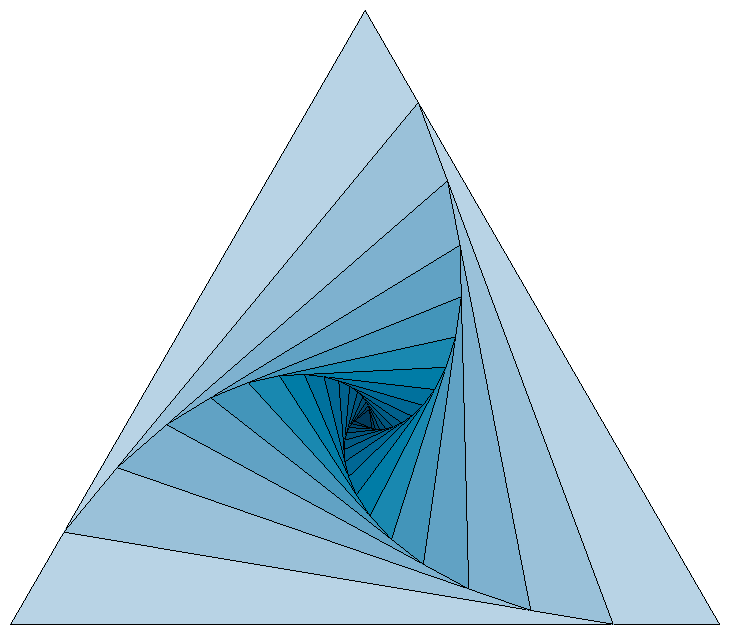
\includegraphics[width=0.35\textwidth]{rotated-triangle}}
\end{figure}
\item Θα ξεκινήσουμε με απλά πράγματα. Για να σχεδιάσετε μια γραμμή στο \en \tikzname:\gr
\vskip 1ex \en
\begin{exampletwouptiny}
\begin{tikzpicture}
\draw (0,0) -- (1,1); % a line
\end{tikzpicture}
\end{exampletwouptiny}
\end{itemize}
\end{frame}
\gr
%%%%%%%%%%%%%%%%%%%%%%%%%%%%%%%%%%%%%%%%%%%%%%%%%%%%%%%%%%%%%%%%%%%%%%%%%%%%%%%
%%%%%%%%%%%%%%%%%%%%%%%%%%%%%%%%%%%%%%%%%%%%%%%%%%%%%%%%%%%%%%%%%%%%%%%%%%%%%%%
%%%%%%%%%%%%%%%%%%%%%%%%%%%%%%%%%%%%%%%%%%%%%%%%%%%%%%%%%%%%%%%%%%%%%%%%%%%%%%%
\begin{frame}[fragile]{\insertsection: Συντεταγμένες}
\begin{itemize}
\item Οι προεπιλεγμένες συντεταγμένες είναι εκατοστά, με τη συνήθη έννοια:
\begin{figure}
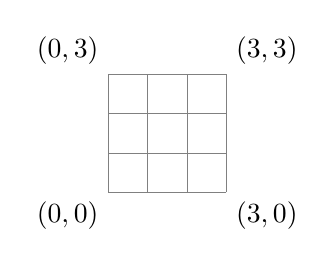
\begin{tikzpicture}[scale=0.5]
\draw[help lines] (0,0) grid (3,3);
\node[below left] at (0,0) {$(0,0)$};
\node[below right] at (3,0) {$(3,0)$};
\node[above right] at (3,3) {$(3,3)$};
\node[above left] at (0,3) {$(0,3)$};
\end{tikzpicture}
\end{figure}
\item Βοηθάει να σχεδιάσετε ένα πλέγμα όταν εργάζεστε με το \en \tikzname:\gr
\vskip 1ex \en
\begin{exampletwouptiny}

\begin{tikzpicture}
\draw[help lines] (0,0) grid (3,3);
\end{tikzpicture}
\end{exampletwouptiny}
\end{itemize}
\end{frame}
\gr
%%%%%%%%%%%%%%%%%%%%%%%%%%%%%%%%%%%%%%%%%%%%%%%%%%%%%%%%%%%%%%%%%%%%%%%%%%%%%%%
%%%%%%%%%%%%%%%%%%%%%%%%%%%%%%%%%%%%%%%%%%%%%%%%%%%%%%%%%%%%%%%%%%%%%%%%%%%%%%%
%%%%%%%%%%%%%%%%%%%%%%%%%%%%%%%%%%%%%%%%%%%%%%%%%%%%%%%%%%%%%%%%%%%%%%%%%%%%%%%
\begin{frame}[fragile]{\insertsection: Γραμμές}
\begin{itemize}
\item Οι αιχμές βελών και τα στυλ γραμμής καθορίζονται ως επιλογές στην εντολή \en \cmdbs{draw}.\gr
\item Τερματίστε κάθε εντολή σχεδίασης με ένα ερωτηματικό \en \keystrokebftt{;}\gr.
\vskip 1ex \en
\begin{exampletwouptiny}
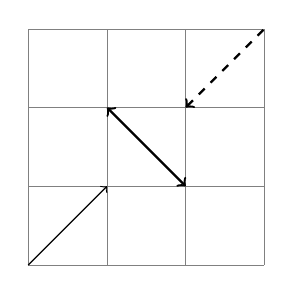
\begin{tikzpicture}
\draw[help lines] (0,0) grid (3,3);
\draw[->] (0,0) -- (1,1);
\draw[<->, thick] (2,1) -- (1,2);
\draw[<-, thick, dashed] (2,2)--(3,3);
\end{tikzpicture}
\end{exampletwouptiny}
\end{itemize}
\end{frame}
\gr
%%%%%%%%%%%%%%%%%%%%%%%%%%%%%%%%%%%%%%%%%%%%%%%%%%%%%%%%%%%%%%%%%%%%%%%%%%%%%%%
%%%%%%%%%%%%%%%%%%%%%%%%%%%%%%%%%%%%%%%%%%%%%%%%%%%%%%%%%%%%%%%%%%%%%%%%%%%%%%%
%%%%%%%%%%%%%%%%%%%%%%%%%%%%%%%%%%%%%%%%%%%%%%%%%%%%%%%%%%%%%%%%%%%%%%%%%%%%%%%
\begin{frame}[fragile]{\insertsection: Μονοπάτια}
\begin{itemize}
\item Μπορείτε να καθορίσετε πολλά σημεία για να σχηματίσετε μια διαδρομή.
\item Τα βέλη θα εμφανίζονται μόνο στα άκρα της διαδρομής.
\vskip 1ex \en
\begin{exampletwouptiny}
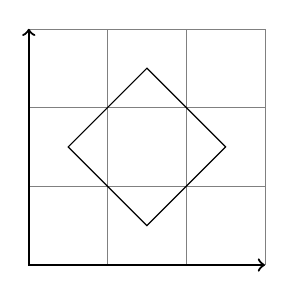
\begin{tikzpicture}
\draw[help lines] (0,0) grid (3,3);
% axes:
\draw[<->, thick] (0,3)--(0,0)--(3,0);
% diamond:
\draw (1.5,0.5) -- (2.5,1.5) -- 
      (1.5,2.5) -- (0.5,1.5) --
      cycle; % close the path
\end{tikzpicture}
\end{exampletwouptiny}
\end{itemize}
\end{frame}
\gr
%%%%%%%%%%%%%%%%%%%%%%%%%%%%%%%%%%%%%%%%%%%%%%%%%%%%%%%%%%%%%%%%%%%%%%%%%%%%%%%
%%%%%%%%%%%%%%%%%%%%%%%%%%%%%%%%%%%%%%%%%%%%%%%%%%%%%%%%%%%%%%%%%%%%%%%%%%%%%%%
%%%%%%%%%%%%%%%%%%%%%%%%%%%%%%%%%%%%%%%%%%%%%%%%%%%%%%%%%%%%%%%%%%%%%%%%%%%%%%%
\begin{frame}[fragile]{\insertsection: Χρώματα}
\begin{itemize}
\item Τα χρώματα καθορίζονται επίσης με την \en \cmdbs{draw}\gr.
\vskip 1ex \en
\begin{exampletwouptiny}
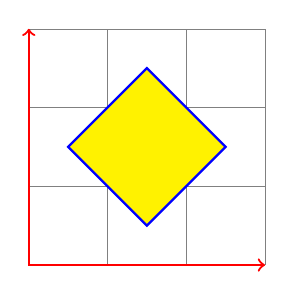
\begin{tikzpicture}
\draw[help lines] (0,0) grid (3,3);
% axes
\draw[<->, thick, red]
  (0,3)--(0,0)--(3,0); 
% diamond
\draw[thick, blue, fill=yellow]
  (1.5,0.5) -- (2.5,1.5) -- 
  (1.5,2.5) -- (0.5,1.5) --
  cycle;
\end{tikzpicture}
\end{exampletwouptiny}
\end{itemize}
\end{frame}

%%%%%%%%%%%%%%%%%%%%%%%%%%%%%%%%%%%%%%%%%%%%%%%%%%%%%%%%%%%%%%%%%%%%%%%%%%%%%%%
%%%%%%%%%%%%%%%%%%%%%%%%%%%%%%%%%%%%%%%%%%%%%%%%%%%%%%%%%%%%%%%%%%%%%%%%%%%%%%%
%%%%%%%%%%%%%%%%%%%%%%%%%%%%%%%%%%%%%%%%%%%%%%%%%%%%%%%%%%%%%%%%%%%%%%%%%%%%%%%
\begin{frame}[fragile]{\insertsection: Σχήματα}
\begin{itemize}
\item Το \en \tikzname{} \gr έχει ενσωματωμένες εντολές για απλά σχήματα.
\vskip 1ex \en
\begin{exampletwouptiny}
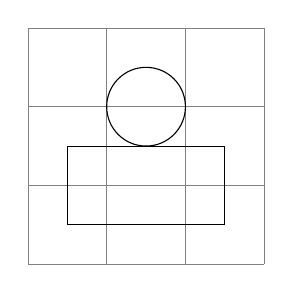
\begin{tikzpicture}
\draw[help lines] (0,0) grid (3,3);
\draw (1.5,2.0) circle (0.5);
\draw (0.5,0.5) rectangle (2.5,1.5);
\end{tikzpicture}
\end{exampletwouptiny}
\end{itemize}
\end{frame}
\gr
%%%%%%%%%%%%%%%%%%%%%%%%%%%%%%%%%%%%%%%%%%%%%%%%%%%%%%%%%%%%%%%%%%%%%%%%%%%%%%%
%%%%%%%%%%%%%%%%%%%%%%%%%%%%%%%%%%%%%%%%%%%%%%%%%%%%%%%%%%%%%%%%%%%%%%%%%%%%%%%
%%%%%%%%%%%%%%%%%%%%%%%%%%%%%%%%%%%%%%%%%%%%%%%%%%%%%%%%%%%%%%%%%%%%%%%%%%%%%%%
\begin{frame}[fragile]{\insertsection: Κόμβοι \& Ετικέτες}
\begin{itemize}
\item Χρησιμοποιήστε κόμβους για να τοποθετήσετε κείμενο (και μαθηματικά) στα σχέδια \en \tikzname{}\gr.
\item Μπορείτε επίσης να χρησιμοποιήσετε κόμβους ως συντεταγμένες --- χρήσιμο για διαγράμματα.
\vskip 1ex 
\en
\begin{exampletwouptiny}
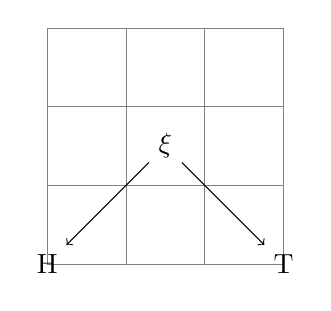
\begin{tikzpicture}
\draw[help lines] (0,0) grid (3,3);
\node (h) at (0,0) {H};
\node (x) at (1.5,1.5) {$\xi$};
\node (t) at (3,0) {T};
\draw[->] (x) -- (h);
\draw[->] (x) -- (t);
\end{tikzpicture}
\end{exampletwouptiny}
\end{itemize}
\end{frame}
\gr
%%%%%%%%%%%%%%%%%%%%%%%%%%%%%%%%%%%%%%%%%%%%%%%%%%%%%%%%%%%%%%%%%%%%%%%%%%%%%%%
%%%%%%%%%%%%%%%%%%%%%%%%%%%%%%%%%%%%%%%%%%%%%%%%%%%%%%%%%%%%%%%%%%%%%%%%%%%%%%%
%%%%%%%%%%%%%%%%%%%%%%%%%%%%%%%%%%%%%%%%%%%%%%%%%%%%%%%%%%%%%%%%%%%%%%%%%%%%%%%
\begin{frame}[fragile]{\insertsection: Συναρτήσεις}
\begin{itemize}
\item Μπορείτε ακόμη και να σχεδιάσετε μερικές απλές συναρτήσεις.
\vskip 1ex \en
\begin{exampletwouptiny}
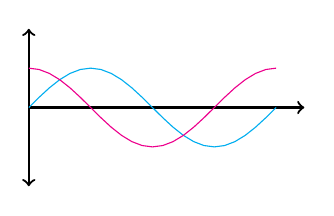
\begin{tikzpicture}[scale=0.5]
% y axis
\draw[<->, thick] (0,2) -- (0,-2);
% x axis
\draw[ ->, thick] (0,0) -- (7, 0); 
% curves
\draw[cyan,domain=0:2*pi]
  plot (\x, {sin(\x r)});
\draw[magenta,domain=0:2*pi]
  plot (\x, {cos(\x r)});
\end{tikzpicture}
\end{exampletwouptiny}
\end{itemize}
\end{frame}

%%%%%%%%%%%%%%%%%%%%%%%%%%%%%%%%%%%%%%%%%%%%%%%%%%%%%%%%%%%%%%%%%%%%%%%%%%%%%%%
%%%%%%%%%%%%%%%%%%%%%%%%%%%%%%%%%%%%%%%%%%%%%%%%%%%%%%%%%%%%%%%%%%%%%%%%%%%%%%%
%%%%%%%%%%%%%%%%%%%%%%%%%%%%%%%%%%%%%%%%%%%%%%%%%%%%%%%%%%%%%%%%%%%%%%%%%%%%%%%
\begin{frame}[fragile]{\insertsection: Παραδείγματα}
\begin{itemize}
\itemΡίξτε μια ματιά στο \en \fbox{\href{http://texample.net/tikz/}{\TeX{}ample.net}} \gr \spaceγια πολλά παραδείγματα \en \tikzname{}:
\end{itemize}
\begin{figure}
\href{http://texample.net/tikz/examples/escher-brick-penrose-triangle/}{%
  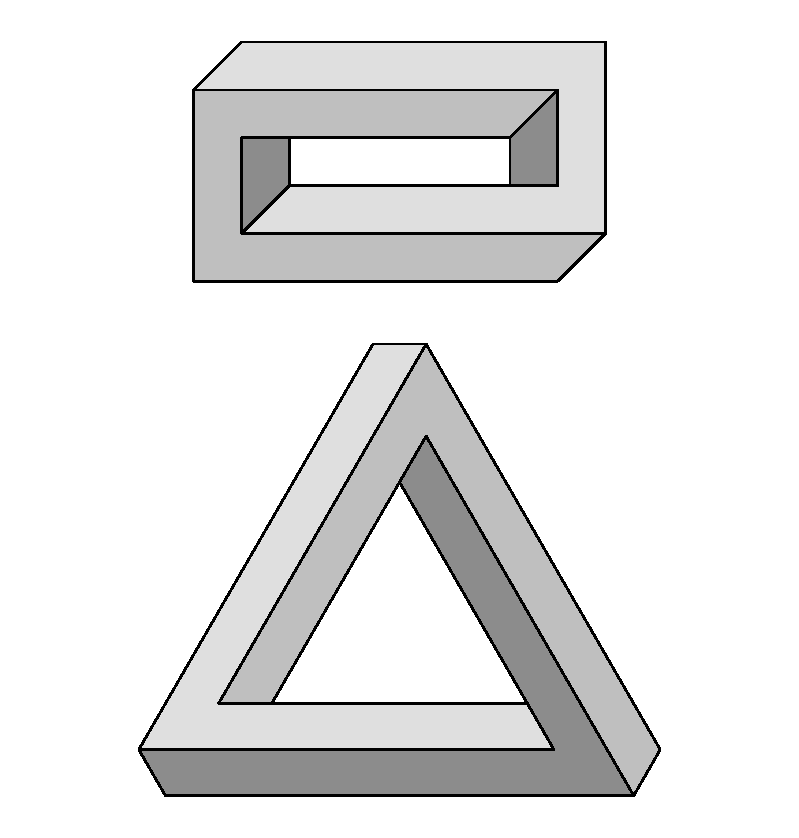
\includegraphics[width=0.3\textwidth]{escher-brick-penrose-triangle}}
\href{http://texample.net/tikz/examples/computer-science-mindmap/}{%
  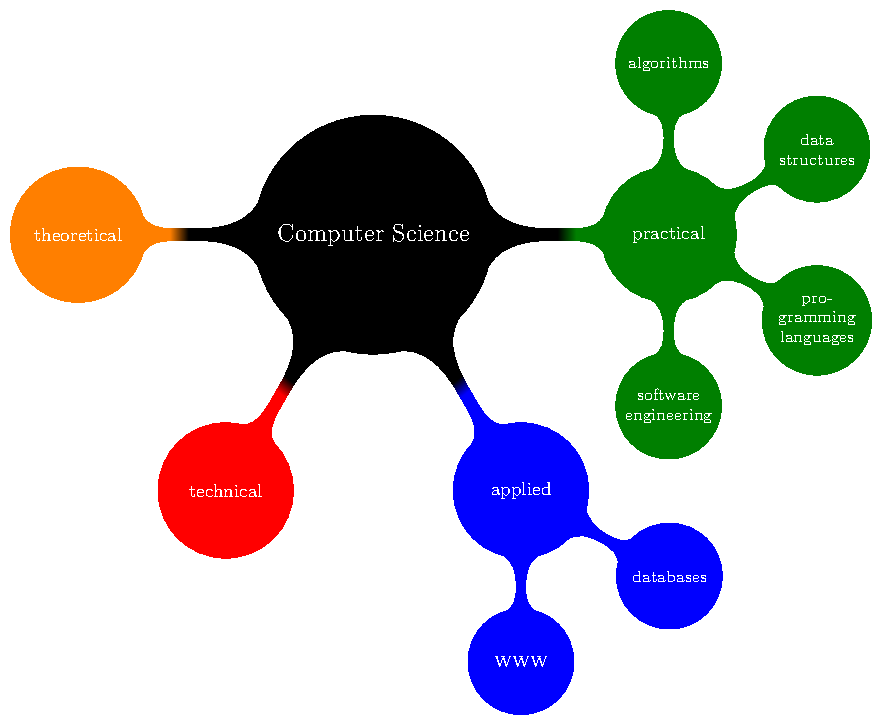
\includegraphics[width=0.3\textwidth]{computer-science-mindmap}}
\href{http://texample.net/tikz/examples/gajski-kuhn-y-chart/}{%
  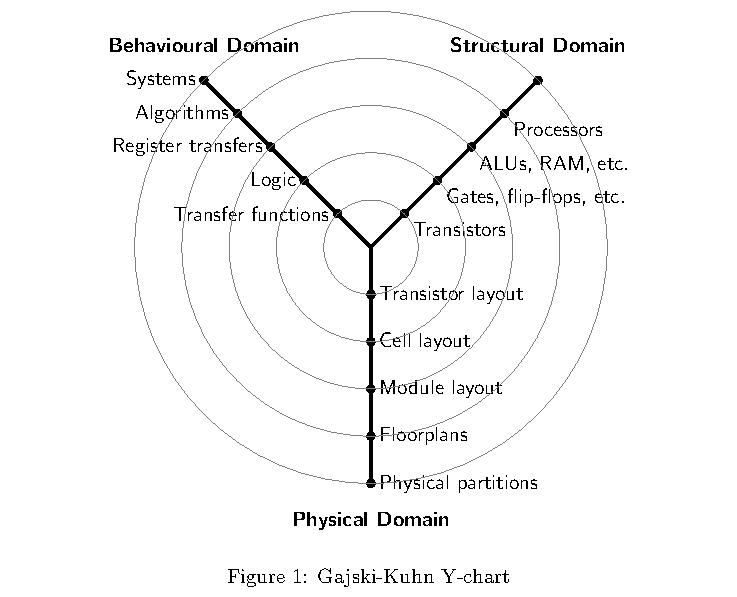
\includegraphics[width=0.3\textwidth]{gajski-kuhn-y-chart}}
\end{figure}
\end{frame}

%%%%%%%%%%%%%%%%%%%%%%%%%%%%%%%%%%%%%%%%%%%%%%%%%%%%%%%%%%%%%%%%%%%%%%%%%%%%%%%
%%%%%%%%%%%%%%%%%%%%%%%%%%%%%%%%%%%%%%%%%%%%%%%%%%%%%%%%%%%%%%%%%%%%%%%%%%%%%%%
%%%%%%%%%%%%%%%%%%%%%%%%%%%%%%%%%%%%%%%%%%%%%%%%%%%%%%%%%%%%%%%%%%%%%%%%%%%%%%%
\begin{frame}[fragile]{\insertsection: Άσκηση}
Σχεδιάστε αυτό με \en \tikzname:\footnote{\gr Βασισμένο στο \en  \url{http://xkcd.com/1022}}
\begin{figure}
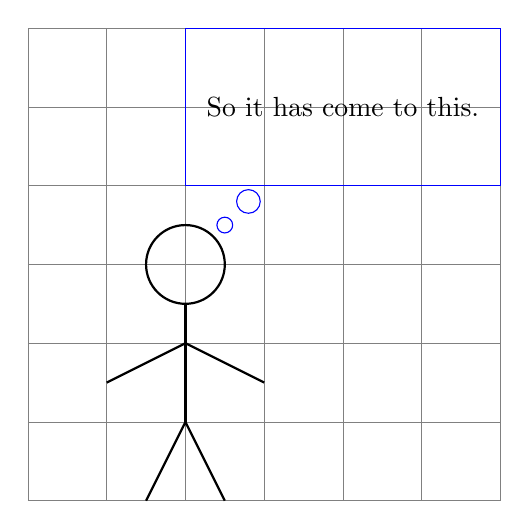
\begin{tikzpicture}
\draw[help lines] (0,0) grid (6,6);
\draw[thick] (2,3) circle (0.5);
\draw[thick] (2,2.5) -- (2,1);              % body
\draw[thick] (1,1.5) -- (2,2) -- (3,1.5);   % arms
\draw[thick] (1.5, 0) -- (2,1) -- (2.5, 0); % legs
\draw[blue] (2,4) rectangle (6,6);
\draw[blue] (2.5,3.5) circle (0.1);
\draw[blue] (2.8,3.8) circle (0.15);
\node at (4,5) {So it has come to this.};
\end{tikzpicture}

\end{figure}
\end{frame}

%%%%%%%%%%%%%%%%%%%%%%%%%%%%%%%%%%%%%%%%%%%%%%%%%%%%%%%%%%%%%%%%%%%%%%%%%%%%%%%
%%%%%%%%%%%%%%%%%%%%%%%%%%%%%%%%%%%%%%%%%%%%%%%%%%%%%%%%%%%%%%%%%%%%%%%%%%%%%%%
%%%%%%%%%%%%%%%%%%%%%%%%%%%%%%%%%%%%%%%%%%%%%%%%%%%%%%%%%%%%%%%%%%%%%%%%%%%%%%%
\section{Σημειώσεις με \protect\en\bftt{ todonotes}}\gr

%%%%%%%%%%%%%%%%%%%%%%%%%%%%%%%%%%%%%%%%%%%%%%%%%%%%%%%%%%%%%%%%%%%%%%%%%%%%%%%
%%%%%%%%%%%%%%%%%%%%%%%%%%%%%%%%%%%%%%%%%%%%%%%%%%%%%%%%%%%%%%%%%%%%%%%%%%%%%%%
%%%%%%%%%%%%%%%%%%%%%%%%%%%%%%%%%%%%%%%%%%%%%%%%%%%%%%%%%%%%%%%%%%%%%%%%%%%%%%%
\begin{frame}[fragile]{\insertsection}
\begin{itemize}
\item Η εντολή \en \cmdbs{todo}\gr από το πακέτο \en \bftt{todonotes}\gr είναι ιδανική για να αφήνετε σημειώσεις στον εαυτό σας και στους συνεργάτες σας. 
\en
\begin{exampletwouptiny}
\todo{add results}
\todo[color=blue!20]{fix method}
\end{exampletwouptiny}
\gr
\vskip 2ex
\item \en Pro Tip:\gr ορίστε τις δικές σας εντολές με \en \cmdbs{newcommand}\gr
\en
\begin{minted}[fontsize=\scriptsize,frame=single]{latex}
\newcommand{\alice}[1]{\todo[color=green!40]{#1}}
\newcommand{\bob}[1]{\todo[color=purple!40]{#1}}
\end{minted}
\gr
Αυτό μπορεί να μας γλιτώσει από πολύ πληκτρολόγηση:
\en
\begin{exampletwouptiny}
\alice{add results}
\bob{fix method}
\end{exampletwouptiny}
\end{itemize}
\end{frame}
\gr
%%%%%%%%%%%%%%%%%%%%%%%%%%%%%%%%%%%%%%%%%%%%%%%%%%%%%%%%%%%%%%%%%%%%%%%%%%%%%%%
%%%%%%%%%%%%%%%%%%%%%%%%%%%%%%%%%%%%%%%%%%%%%%%%%%%%%%%%%%%%%%%%%%%%%%%%%%%%%%%
%%%%%%%%%%%%%%%%%%%%%%%%%%%%%%%%%%%%%%%%%%%%%%%%%%%%%%%%%%%%%%%%%%%%%%%%%%%%%%%
\begin{frame}[fragile]{\insertsection}
\begin{columns}
  \begin{column}{0.4\textwidth}
    \begin{itemize}
    \item Μόνο οι ενσωματωμένες σημειώσεις υποστηρίζονται στο \en beamer\gr, αλλά οι σημειώσεις περιθωρίου υποστηρίζονται για κανονικά έγγραφα.
    \item Υπάρχει επίσης μια εύχρηστη εντολή \en \cmdbs{listoftodos}\gr.
    \end{itemize}
  \end{column}
  \begin{column}{0.6\textwidth}
    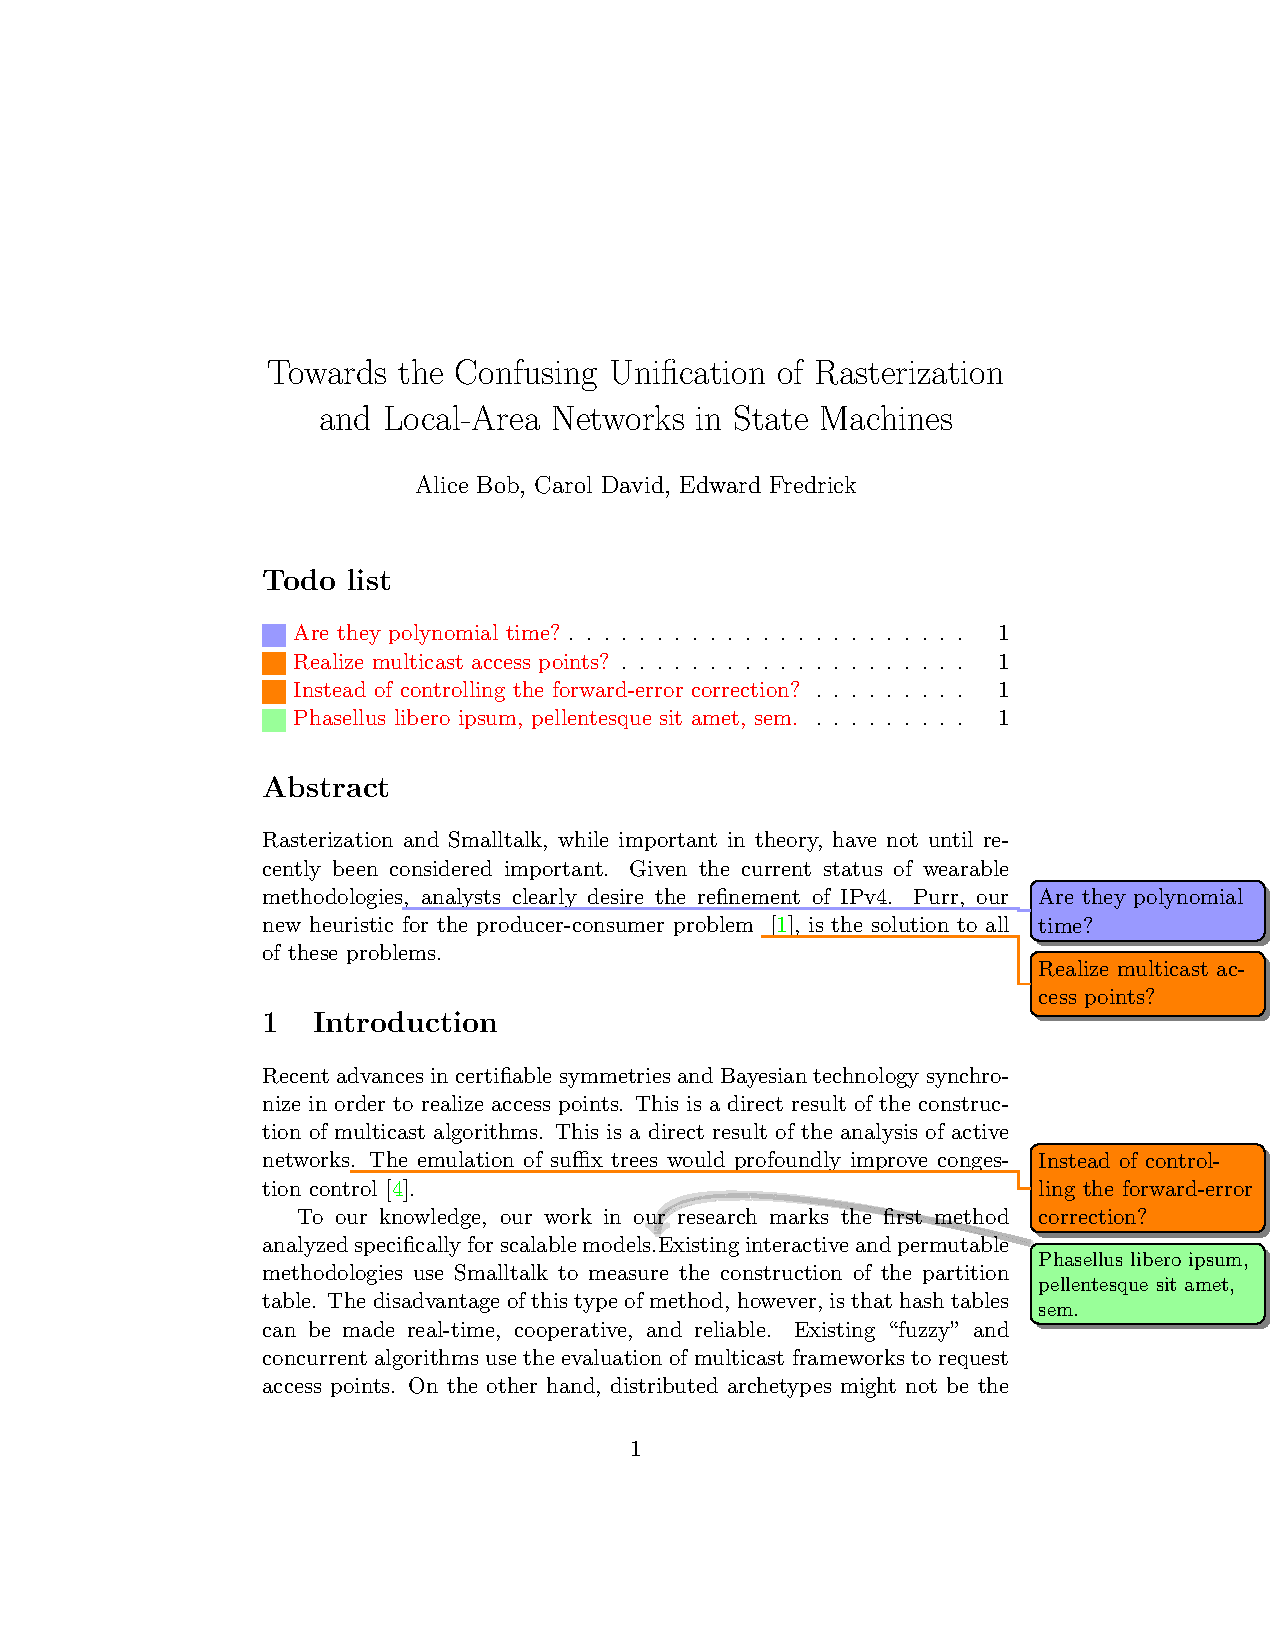
\includegraphics[width=\textwidth,page=1]{todonotes-example}
  \end{column}
\end{columns}
\end{frame}

%%%%%%%%%%%%%%%%%%%%%%%%%%%%%%%%%%%%%%%%%%%%%%%%%%%%%%%%%%%%%%%%%%%%%%%%%%%%%%%
%%%%%%%%%%%%%%%%%%%%%%%%%%%%%%%%%%%%%%%%%%%%%%%%%%%%%%%%%%%%%%%%%%%%%%%%%%%%%%%
%%%%%%%%%%%%%%%%%%%%%%%%%%%%%%%%%%%%%%%%%%%%%%%%%%%%%%%%%%%%%%%%%%%%%%%%%%%%%%%
\section{Υπολογιστικά φύλλα με \en \protect\bftt{spreadtab}}\gr

%%%%%%%%%%%%%%%%%%%%%%%%%%%%%%%%%%%%%%%%%%%%%%%%%%%%%%%%%%%%%%%%%%%%%%%%%%%%%%%
%%%%%%%%%%%%%%%%%%%%%%%%%%%%%%%%%%%%%%%%%%%%%%%%%%%%%%%%%%%%%%%%%%%%%%%%%%%%%%%
%%%%%%%%%%%%%%%%%%%%%%%%%%%%%%%%%%%%%%%%%%%%%%%%%%%%%%%%%%%%%%%%%%%%%%%%%%%%%%%
\begin{frame}[fragile]{\insertsection}
\begin{itemize}
\item
Τώρα που είδατε πώς το \LaTeX{} μπορεί να αντικαταστήσει το \en Word \gr και το \en PowerPoint, \gr τι γίνεται με το \en Excel;\gr
\item Εργασία για το σπίτι: δοκιμάστε το \fbox{\href{http://www.ctan.org/pkg/spreadtab}{\en \bftt{spreadtab} \gr πακέτο}}!
\end{itemize}
\end{frame}

%%%%%%%%%%%%%%%%%%%%%%%%%%%%%%%%%%%%%%%%%%%%%%%%%%%%%%%%%%%%%%%%%%%%%%%%%%%%%%%
%%%%%%%%%%%%%%%%%%%%%%%%%%%%%%%%%%%%%%%%%%%%%%%%%%%%%%%%%%%%%%%%%%%%%%%%%%%%%%%
%%%%%%%%%%%%%%%%%%%%%%%%%%%%%%%%%%%%%%%%%%%%%%%%%%%%%%%%%%%%%%%%%%%%%%%%%%%%%%%
\begin{frame}
\begin{center}
Ευχαριστώ, και χαρούμενο  \TeX{}\en ing \gr!
\end{center}
\end{frame}

\end{document}
